%% This is an example first chapter.  You should put chapter/appendix that you
%% write into a separate file, and add a line \include{yourfilename} to
%% main.tex, where `yourfilename.tex' is the name of the chapter/appendix file.
%% You can process specific files by typing their names in at the 
%% \files=
%% prompt when you run the file main.tex through LaTeX.
\chapter{Introduction}\label{intro-ch}

Many applications require a domain expert to visually inspect and process a
dataset on a stream of incoming data. The problem with such manual inspection
is it's inability to scale as datasets grow exponentially \cite{exp-growth}. As
the data set grows, it becomes difficult to visualize and interact with
\cite{immens} and there are also many cases of false positives which the expert
should not have to manually reclassify. We with to focus on the field of
medical data, where doctors have to view a patient's data and extract relevant
information for treatment. Specifically, we focus on electroencephalogram (EEG)
readings, a test which is used to detect abnormalities related to the
electrical activity of the brain. \\

Today, doctors are faced with having to store large amounts of patient data
without analysis since they lack the tools to efficiently view datasets are a
large scale. To remedy this, we have designed and implemented a system, Pinky,
which can process large amounts of EEG data, allowing near real-time
interaction for analysis.


\section{Pinky}

Pinky is a doctor's newest tool for analysing the brain, see Figure
\ref{fig:pinky-and-the-brain}. Working with a team of researchers at
Massachusetts General Hospital, we have designed and implemented the system to
handle the fast growing corpus of EEG data that is being collected. This
end-to-end system handles the storage, computation, and visualization of EEG.
The goal of the system is to provide a scalable architecture for concurrent
analysis of patient records with near real time interactivity. Each layer of
the system has been optimized for use and evaluated across hundreds of GB of
patient data. \\

\begin{figure}[h]
\begin{center}

\includegraphics[scale=0.75]{./img/pinky-and-the-brain.png}
\caption{Etymology of Pinky's name.}
\label{fig:pinky-and-the-brain}
\end{center}
\end{figure}

\section{Overview of EEG Analysis}

TODO:
What is EEG analysis? Why is it important? What is the scale of the problem? How have we fixed it?

\section{System Architecture}

The system is comprised of three coupled layers which handle, storage,
computation and visualization. Figure \ref{fig:system-architecture} shows the
overall architecture of the system.

\begin{figure}[h]
\begin{center}
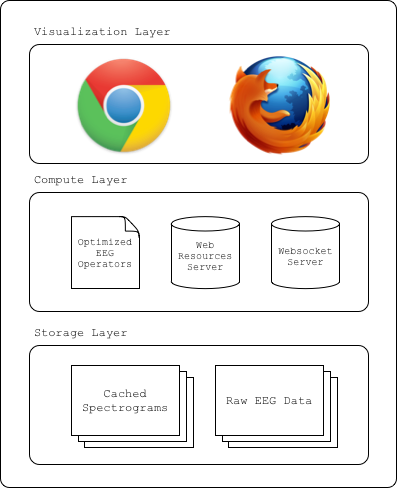
\includegraphics[scale=0.7]{./img/system-architecture.png}
\caption{Pinky System Architecture.}
\label{fig:system-architecture}
\end{center}
\end{figure}

\subsection{Storage Layer}

The storage layer, discuss in detail in chapter \ref{storage-ch}, is responsible for
storing raw EEG patient data and a copy of the calculated spectrogram. This
datastore must be optimized for both reads and writes of array based data for
multidimensional arrays on the order to tens to hundreds of GB.

\subsection{Compute Layer}

The compute layer, discuss in detail in chapter \ref{compute-ch}, is meant to be an
extendible module which handles the algorithms to calculate the spectrogram and
other EEG related calculations. As we discuss in \ref{discuss-ch:future-work},
there are several extensions the project can take, thus it is important that an
interested developer can easily add functionality to this layer. In addition,
the compute layer contains two servers, one to server the array based data,
interfacing with the optimized EEG algorithms, and a lightweight server for the
web resources to be served to the visualization layer.

\subsection{Visualization Layer}

The visualization layer, discussed in detail in chapter \ref{viz-ch}, is a browser
based module that renders the data to the client. The interface allows users to
query based on a patient's id (medical record number, \c{mrn}) and view a spectrogram
for a given time interval.

\subsection{Visgoth System}

Since enabling interactivity is an important design criteria, we have designed
and built a optimization module for time series visualization in the browser,
Visgoth. This is discussed in detail in chapter \ref{visgoth-ch}.

\section{Usage}

The project code base is available publicly on Github \cite{github}
\url{https://github.com/joshblum/eeg-toolkit} with documentation for installing
the project for development. In addition, we have created Docker \cite{docker}
images that can easily be install for production use. Armed with a dataset, any
curious doctor should be able to install the images and load the data for
analysis. The docker images are available for public use here:
\url{https://hub.docker.com/r/joshblum/eeg-toolkit-webapp} and
\url{https://hub.docker.com/r/joshblum/eeg-toolkit-toolkit}. Specific
installation instructions can be found with the github project.

\section{Contributions}

Pinky make several contributions:

\begin{itemize}
  \item Implements an abstraction for array based storage systems.
  \item Implements 4 different backends to adhere to the abstraction.
  \item Evaluates the different backends for multiple input ranges and workloads.
  \item Implements optimized algorithms for analysing EEG data.
  \item Provides an extendible framework for accessing array based data and visualizing it in the browser.
  \item Implements scalable in-browser visualizations using the client's GPU.
  \item Implements a new system, Visgoth, for reducing latency for time series based visualizations.
\end{itemize}

These contributions enable doctors and medical expert analysts to interactively
analyse EEG data at scale.

